\chapter{反三角函数与简单三角方程的解法}
\section{反正弦函数}
我们知道,正弦函数$y=\sin x$是一个周期等于$2\pi$的振动函
数,它的定义域是$(-\infty,+\infty)$, 而值域是闭区间$[-1,1]$, 它的图象如图9.1。

\begin{figure}[htp]
    \centering
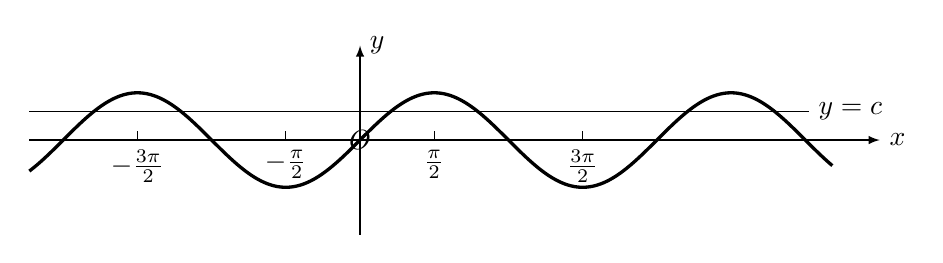
\begin{tikzpicture}[>=latex, scale=.6]
\draw[->] (-7,0)--(11,0)node[right]{$x$};
\draw [->] (0,-2)--(0,2)node[right]{$y$};

\draw[domain=-7:10, samples=1000, very thick] plot(\x,{sin(\x r)});
\draw  (-7,.6)--(9.5,0.6)node[right]{$y=c$};

\foreach \x/\xtext in {-1.5*pi/-\frac{3\pi}{2}, -.5*pi/-\frac{\pi}{2},.5*pi/\frac{\pi}{2}, 1.5*pi/\frac{3\pi}{2}}
{
    \draw (\x,0)node[below]{$\xtext$}--(\x,.2);
}
\node(.5,-.5){$O$};
\end{tikzpicture}
    \caption{}
\end{figure}


每取一数$y=c,\; -1\le c\le 1$, 作直线$y=c$, 可与正弦曲线
$y=\sin x$交于无穷多个点,这些交点的横坐标是
\[x=x_0+2k\pi\qquad \text{和}\qquad x=(π-x_0)+2k\pi\quad (k\in\mathbb{Z})\]
因此有无数多个$x$的值满足方程$\sin x =c$, 而和那个$y=c$对
应。可见对于变数$x$的一切可能实数值来说,我们不能由函
数$f:\mathbb{R}\to [-1,1]$, $f(x)=\sin x$得出它的反函数来。把定
义域分成无数个单调区间,则在各区间$\left[-\frac{\pi}{2}+2k\pi, \frac{\pi}{2}+2k\pi\right]$上,$y=\sin x$由$-1$上升到1,而在各区间$\left[\frac{\pi}{2}+2k\pi, \frac{3\pi}{2}+2k\pi\right]$上,$y=\sin x$由1下降到$-1$,于是由前一章中的
反函数定理知道,对于上述每一个单调区间存在一个反函数。

如果我们强调的是在闭区间$\left[-\frac{\pi}{2},\frac{\pi}{2}\right]$上
来考虑正弦
函数的反函数,我们就说它是反正弦函数的主值,并把这个函数记作
$x=\arcsin y$,使得
$$x=\arcsin y\qquad \Longleftrightarrow \qquad y=\sin x$$
这里$x\in \left[-\frac{\pi}{2},\frac{\pi}{2}\right],\quad y\in[-1,+1]$。

对于使得$y=\sin x$是单调的另一区间,例如$x\in \left[\frac{\pi}{2},\frac{3\pi}{2}\right]$,
我们就得到另一个反正弦函数。假如我们没有明确地
指出反正弦函数的值域所在的区间,我们就不能由函数$y=\sin x$得出它的反函数。为了明确起见,现在我们规定

\begin{blk}{定义1}
    函数$y=\sin x$在闭区间$\left[-\frac{\pi}{2},\frac{\pi}{2}\right]$上
的反函数
叫做\textbf{反正弦函数}或\textbf{反正弦},这个函数用记号写作
$x=\arcsin y$ (即$x$是一角或弧,其相应的正弦值为$y$),
它的定义域是闭区间$-1\le y\le 1$, 值域是闭区间$-\frac{\pi}{2}\le x\le \frac{\pi}{2}$。
\end{blk}

用习惯上的写法,将字母$x$与$y$互换而写成$y=\arcsin x$,
现在,我们将反正弦函数(主值)的定义用几何名词叙述
如下:

在闭区间$-1\le x\le 1$上,数$x$的反正弦$y=\arcsin x$是在
闭区间$\left[-\frac{\pi}{2},\frac{\pi}{2}\right]$上
的一个角或弧,它的正弦值等于$x$, 
即$\sin y=x$.

由反正弦函数的定义和前一章的反函数定理可得到
它的一些性质如下:





















































































\section*{习题9.1}
\addcontentsline{toc}{subsection}{习题9.1}
\begin{enumerate}
    \item 用反三角函数表示下面等式中的角。
    \begin{multicols}{2}
\begin{enumerate}
    \item $\sin\frac{\pi}{4}=\frac{\sqrt{2}}{2}$
    \item $\sin\frac{5\pi}{3}=-\frac{\sqrt{3}}{3}$
    \item $\sin\frac{7\pi}{3}=\frac{\sqrt{3}}{2}$
    \item $\sin(-2.314)=-0.04038$
\end{enumerate}
    \end{multicols}
    \item 当$\frac{1}{2}\le x\le\frac{\sqrt{3}}{2}$
    时,求函数$y=x\arcsin x$的最大值
    和最小值。
    \item 不求值,确定下面差的符号:
\begin{enumerate}
    \item $\arcsin 0.7-\arcsin 0.5$
    \item $\arcsin\left(-\frac{3}{5}\right)-\arcsin\left(-\frac{3}{4}\right)$
    \item $\arcsin\left(\sqrt{2}-1\right)-\arcsin\left(\sqrt{5}-2\right)$
\end{enumerate}
\item 求下列各式的值:
\begin{multicols}{2}
\begin{enumerate}
    \item $\arcsin\frac{\sqrt{3}}{2}$
    \item $\arcsin\left(-\frac{\sqrt{2}}{2}\right)$
    \item $\arcsin0$
    \item $\arcsin(-1)$
    \item $\arcsin\left(-\frac{1}{4}\right)$
    \item $\arcsin0.7841$
\end{enumerate}
\end{multicols}

\item 计算下列各式的值:
\begin{multicols}{2}
    \begin{enumerate}
        \item $\tan\left(\arcsin\frac{\sqrt{2}}{2}\right)$
        \item $\cos\left(\arcsin \frac{3}{5}\right)$
        \item $\arcsin \left[\sin\left(-\frac{\pi}{7}\right)\right]$
        \item $\arcsin\left(\sin\frac{5\pi}{6}\right)$
        \item $\arcsin(\cos1)$
    \end{enumerate}
    \end{multicols}
    \item 计算下列各式的值:
\begin{multicols}{2}
    \begin{enumerate}
        \item $\cot\left(2\arcsin\frac{\sqrt{2}}{2}\right)$
        \item $\cos\left(2\arcsin\frac{1}{3}\right)$
        \item $\sin\left(3\arcsin\left(-\frac{\sqrt{3}}{2}\right)\right)$
        \item $\tan\left(\frac{1}{2}\arcsin\frac{2}{3}\right)$
    \end{enumerate}
    \end{multicols}

    \item 讨论函数$y=x \arcsin(\sin x)$的图象,并作草图。
\item 画出$f(x)=\sin(3\arcsin x)$的图象。
\end{enumerate}